\RequirePackage{fix-cm}
\documentclass[twocolumn]{svjour3}[]

\smartqed  % flush right qed marks, e.g. at end of proof

\usepackage{graphicx}
\usepackage{xeCJK}
\usepackage{hyperref}
\usepackage{xcolor,colortbl}
\usepackage{ulem}
% \usepackage{titlesec}

% related to table
\usepackage{multirow}
\usepackage{hhline}
\usepackage{booktabs,array,times}

%\setCJKmainfont{BabelStone Han}

\begin{document}

\newcolumntype{Y}{>{\centering\arraybackslash\columncolor{lightgray}}c}
\newcolumntype{Z}{>{\centering\arraybackslash\columncolor{lightgray}}m{0.14\linewidth}}
\newcolumntype{C}{>{\columncolor{lightgray}}c}
\renewcommand{\arraystretch}{1.5}

\title{一种规范的实现敏捷开发实践的方法:敏捷开发框架}

\author{Ahmed Sidky \and James Arthur \and Shawn Bohner}

\institute{S. Bohner \at  Virginia Tech, Blacksburg, VA, USA \\ \email{sbohner@vt.edu} \and
           A. Sidky \at \email{asidky@vt.edu} \and
           J. Arthur \at \email{arthur@vt.edu}
}

\date{Received: 6 March 2007 / Accepted: 8 May 2007 / Published online: 24 July 2007}

\maketitle

\begin{abstract}
很多公司期望应用敏捷开发来利用它所带来的多种优势。这些优势包括更快的投资回报率、更高的软件质量和更高的客户满意度,当然其带来的好处不仅仅是局限于此。然而,到目前为止没有一种结构化的处理方式来指导公司如何实践敏捷开发。为了解决这个问题,我们提出了一种敏捷应用框架和我们已经用于实现它的一些使用方法。这个框架包含两个组件:敏捷测量指数和四阶段处理方法。这两个组件可以很好的指导和帮助公司的敏捷化尝试。更具体来说,Sidky敏捷测量指数(SAMI)包括五个敏捷等级,这五个等级用于指示项目或公司的敏捷潜力。另一方面来说,四阶段方法帮助企业判定是否已经准备好应用敏捷开发,并且根据他们的潜力,那种敏捷实践应该被引入来进行指导。为了帮助证明敏捷开发框架的优势,我们向很多的敏捷社区介绍了这种框架,并通过调查表的方式获取回复。结果是鼓舞人心的,同时我们也会在这篇论文中展示结果。
\end{abstract}

\section{Introduction}
\label{intro}
在过去的几年中,一些企业问敏捷社区:“为什么我们需要采用敏捷实践?”\cite{highsmith2006agile}。这个问题有很多相关的答案,非常多的成功故事都强调了企业在成功应用敏捷开发后所获得的好处\cite{barnett2006agile,barnett2004adopting,kuppuswami2003effects,law2005effects,schatz2005primavera,williams2000strengthening}。因此,很多公司现在期望采用敏捷实践。然后,再一次他们转向敏捷社区,但是这次带着的是不同的问题:“我们怎么做才能应用敏捷实践?”\cite{highsmith2006agile}。但不幸的是,没有任何一种结构化的敏捷实践方法(至少是公开的网站中)。对于想要敏捷化的企业指导和帮助的缺乏是这篇论文主要解决的问题。

造成这种缺乏的一个主要因素是为了成功应用敏捷实践时向企业提供指导时,有很多问题需要这种结构化方法来解决。他们包括:(1)企业对敏捷化的兴趣(2)应该采用的实践方式(3)在应用过程中可能的遇到的困难(4)对敏捷实践应用企业所做的必要准备。

本文介绍的这种敏捷应用框架通过提供一种结构化的、可重复的方法,是解决上面提到的问题的一种尝试。这个框架可以为了协助敏捷社区为日益增长的,想要采用敏捷实践的企业提供支持。

这个敏捷开发框架包括两个主要部件:(1)一个估计敏捷潜力的测算指数(2)一个四阶段的处理方法,使用了测算指数来判断目前的进行到什么程度,什么样的敏捷实践可以被引入。图片\ref{overview}描述了这个框架的不同组件和它们之间的关系。

\begin{figure} [htb]
    \centering
    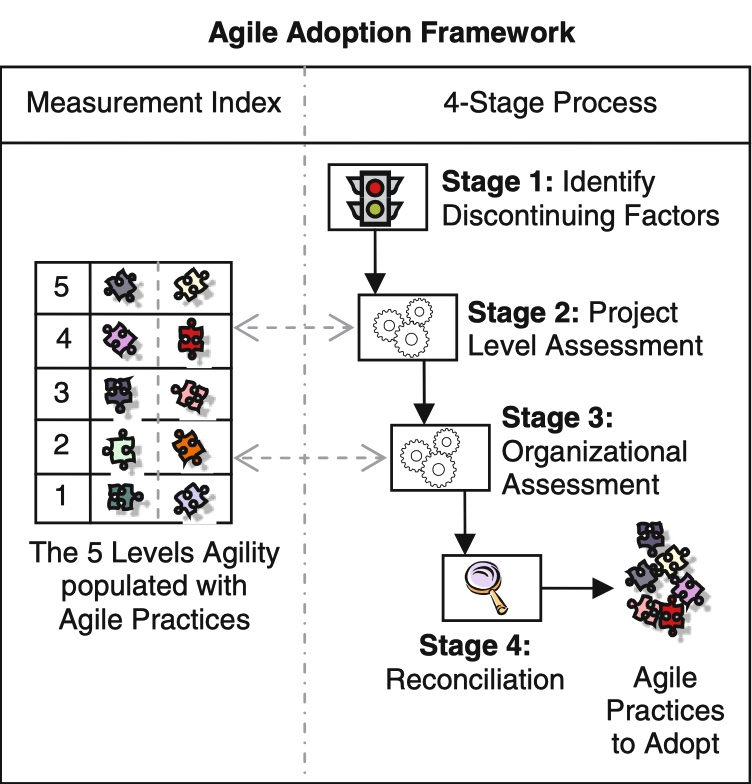
\includegraphics[width=1.0\linewidth]{img/overview.jpg}
    \caption{Overview of the agile adoption framework}
    \label{overview}
\end{figure}

第一个组件名字为Sidky敏捷测算指数(SAMI),它是一个范围用于鉴别一个项目或者一个组织的敏捷潜能。SAMI是用于框架的处理组件中,在该框架中这四种状态相互作用来指导企业找到最适合他们环境的敏捷实践。这四种阶段是:

\begin{itemize}
    \item[$\bullet$] \textit{阶段1:中断因素识别。}发现任何“显式阻塞”的存在,这些“现实阻塞”可以导致采用过程失败。
    \item[$\bullet$] \textit{阶段2:项目阶段评估。}利用SAMI来判定某一项目的敏捷化的目标等级。
    \item[$\bullet$] \textit{阶段3:组织准备程度评估。}使用SAMI来评估企业在多大程度上实现为项目确定的目标敏捷化级别。
    \item[$\bullet$] \textit{阶段4:协调。}通过协调项目的目标敏捷化级别(源自阶段2)和实施组织的准备情况(源自阶段3)判定最终采用的一系列敏捷实践。
\end{itemize}

正如上面列出的那样,敏捷开发框架提供了一种重要的可以保证采用敏捷实践成功的办法,但是只是这一个是远远不够的。在四阶段中的指导和测算的解释要素也是很重要的,或许可以通过一个有经验的敏捷指导师或者一个有着丰富敏捷方法的训练和使用这个框架的内部员工实现。

% TODO
本文的剩余部分会展示敏捷开发框架和提供从行业互动中获得的见解来证明我们的工作。章节\ref{ami}中介绍一种结构和SAMI的详情。

\section{Agile measurement index}
\label{ami}

当寻求应用敏捷实践时,企业有的其中一个顾虑是确定他们可以变得多么敏捷\cite{sidky2007disciplined}。项目或企业的敏捷潜力(即该实体采用敏捷的程度)被他们周围的环境所影响。为了决定敏捷潜力,指导师或者执行评估的人需要一些测算指数或者范围来测算实体的敏捷化水平。在敏捷开发框架中是使用SAMI作为这个标尺的。

敏捷开发框架使用SAMI来确定项目或企业的敏捷潜力。SAMI是一个包含四部分的敏捷测算指数:

\begin{enumerate}
    \item 敏捷级别:当应用敏捷开发时,一组相关的并且可以在软件开发过程中产生重大提升的敏捷实践,从而实现了敏捷化的核心价值
    \item 敏捷原则:需要被应用的准则,以确保开发过程是敏捷的
    \item 敏捷实践和概念:用于以符合敏捷原则的方式开发和管理项目的具体技术和实用技术
    \item 指示器:评估员为了评估企业或项目的某些特征所使用的一些问题,例如其人员、文化和环境,为了评估应用敏捷实践的企业或项目的准备情况。
\end{enumerate}

% TODO
章节\ref{al}-\ref{ap}

\subsection{Agile levels}
\label{al}

\begin{figure*} [htb]
    \centering
    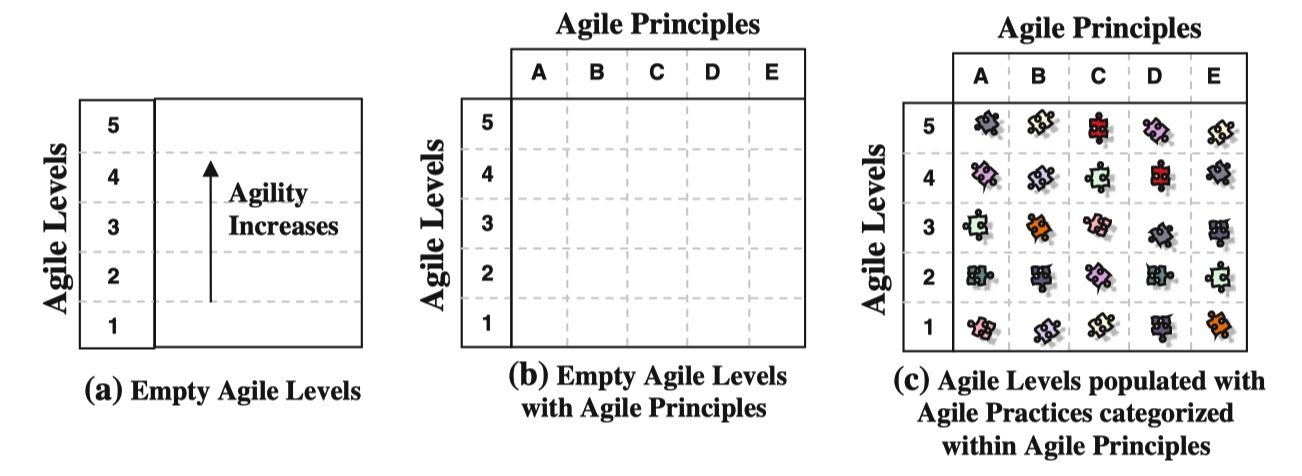
\includegraphics[width=1.0\textwidth]{img/sami-components.jpg}
    \caption{Components of the SAMI (indicators are not shown)}
    \label{sami-com}
\end{figure*}

图片\ref{sami-com}描述了敏捷级别,它被认为是测量尺度的单位,因为他能列举对一个项目或组织的不同且可能的敏捷化程度。这个项目或企业的敏捷潜力表明了它可以达到的最高敏捷程度。到达的特定级别意味着项目和企业已经实现并接受了敏捷开发过程所需要的基本元素。例如,当加强沟通和合作的固有要素体现在开发过程中时,那么敏捷级别1(合作)就达到了。但是,在移动到级别2之前,所有与敏捷级别1有关联的全部实践必须实现。

敏捷化的五个等级用来代表了敏捷宣言的核心特征\cite{agilemanifestoo2001agile},这些特征不与任何特定敏捷方法相关。在自己分析这些宣言后,找出了五个基本的敏捷特征。这些特征构成了SAMI使用的五个敏捷化等级。

\begin{itemize}
    \item[$\bullet$] 级别1:合作。这一级表示促进全部参与者之间的交流和协作。协作的规模是敏捷软件开发的基础\cite{cockburn2001agile,cockburn2001agilesoftware,tabaka2006collaboration}。
    \item[$\bullet$] 级别2:进化。进化开发是\textit{软件的早期和持续交付}。同时它也是基础性的,因为每一个敏捷方法都以它的存在为前提\cite{larman2004agile}。
    \item[$\bullet$] 级别3:效率。这一级关注的是通过应用\textit{工程实践}来增加开发过程的效率,从而\textit{开发出高质量的工作软件}。这需要为下一级的开发过程做准备,在下一级中可以响应持续的改变而不对已经开发的的软件系统造成危害\cite{cockburn2001agilesoftware,hunt2006agile}。
    \item[$\bullet$] 级别4:适应。这一级构成了在开发过程中响应变化的敏捷特性的建立。对多个级别的反馈的定义和响应对这级是非常重要的\cite{highsmith2002agile}。
    \item[$\bullet$] 级别5:包容。敏捷化本质上是一种文化,并且有一个对软件开发过程的敏捷本质支持的环境是很重要的。为了在整个企业中保持并且培育这中敏捷性,这一层聚焦于建立一个\textit{全方位的环境}。
\end{itemize}

每一个敏捷级别都包含了一组推行并保持与该级别相关的敏捷特性的敏捷实践。分配给每个敏捷级别的敏捷实践和敏捷概念的选择是通过测算指数的第二部分\textit{(敏捷原则)}来进行指导的。

\subsection{Agile principles}
\label{ap}

在被认为是\textit{敏捷的}之前,敏捷原则是必须反映到流程中的基本特性。例如,两个关键的敏捷原则是\textit{以人为本}和\textit{技术卓越},其中\textit{以人为本}是指对人的依赖并且在人之间的相互作用,\textit{技术卓越}是指尽可能的产生或维持高质量的代码质量。敏捷宣言列出了12项描述敏捷开发流程的原则\cite{cockburn2001agile}。在进行任重的归纳和总结后,发现了体现12个本质的五个敏捷原则。这五个原则指导了敏捷华的五个级别的改进和修剪。

\begin{itemize}
    \item[$\bullet$] \textit{拥抱变革来实现客户价值\cite{beck2000extreme}。}软件开发工作的成功取决于它在多大程度上帮助实现用户价值的。在许多情况下,为了实现额外客户价值的需求开发团队和顾客都是在不断学习的。因此,在整个软件开发中需要对变化怀着欢迎的态度。
    \item[$\bullet$] \textit{经常规划和交付软件\cite{beck2001manifesto,Cohn:2005:AEP:1036751,rosenberg2005agile}。}软件的早期和频繁交付是很重要的,因为它可以提供给顾客一些用来检查和提供反馈的产品的部分功能部件。对于即将到来的迭代规划过程,这种反馈是很重要的,因为它形成了软件开发工作的范围和方向。
    \item[$\bullet$] \textit{以人为本\cite{cockburn2001agile}。}人员的依赖和他们之间的相互作用是敏捷软件流程的定义中的基石。
    \item[$\bullet$] \textit{技术卓越\cite{highsmith2002agile,koch2005agile}。}敏捷开发人员只能致力于生产最高质量的代码,因为在高速开发环境中高质量代码是非常重要的,例如敏捷开发环境。
    \item[$\bullet$] \textit{客户协作\cite{beck2001manifesto}。}从原始的敏捷宣言的陈述中获得灵感,必须在顾客、开发者和项目参与者之间保持大量且频繁的交流,这样才能保证产品是在满足客户的业务需求的前提下开发的。
\end{itemize}

事实上,敏捷原则被用于确保敏捷级别体现的敏捷化的基本特征。图片2b描述了敏捷级别和敏捷原则之间的关系。每一个敏捷级别应该包含与敏捷实践相关的大部分的敏捷原则。这些原则反映了敏捷实践用于促进与该级别相关的敏捷质量的方法。例如,等级3(效率)的全部实践促进了\textit{在高效的方式下的}开发\textit{高质量的}、\textit{可工作的}软件的敏捷目标。但是,这一目标的实现是由与包含每一级别的敏捷原则的实践决定的。同样,与\textit{技术卓越}相关的实践将会通过聚焦于增强流程的技术方面来实现它的敏捷目标,而与\textit{以人为本}原则相关的实践则是帮助增强流程的人性方面。

然而,SAMI的本质是它所阐述的敏捷实践。下一部分要介绍敏捷化的五个级别的第三个组件——\textit{敏捷实践}。

\subsection{Agile practices}
\label{apract}

敏捷实践是一些在以符合敏捷原则的方式开发和管理软件项目的具体活动和实践技术。例如,\textit{结对开发},\textit{用户故事},和\textit{写作规划}都是敏捷实践。因为敏捷级别是由敏捷实践构成的(按照敏捷原则组织——见图2c),他们都被认为是敏捷测算指数的基础构件。仅在与这个级别相关的敏捷实践被采用时,才能算到达了这个敏捷级别。

在调查了现在被应用于工业中的敏捷方法后\cite{abrahamsson2002agile,hunt2006agile,koch2005agile},40种不同的敏捷实践被用来构成SAMI。这些实践按照敏捷级别和实践排列的,如表\ref{five-levels}所示。(目前带有下划线的实践可以忽略,这些将在论文的后面讨论。)尽管关于每一个敏捷实践和概念的详细讨论都在这篇论文的外部,但是与每一个敏捷实践和概念有关的引用都是更好了解它们的一个很好的起点。

\begin{table*}[!htb]
\centering
\caption{The five levels of agility populated with agile practices and concepts}
\label{five-levels}
\begin{tabular}{|p{0.13\linewidth}|p{0.14\linewidth}|p{0.14\linewidth}|p{0.14\linewidth}|p{0.14\linewidth}|p{0.14\linewidth}|}
    % >>> row 1
    \hline
    \multirow{2}{*}{} & \multicolumn{5}{C|}{\textbf{敏捷原则}} \\ \hhline{|~|-----|}
    
    % >>> row 2
    &
    % c2
    \multicolumn{1}{Z|}{\textit{拥抱变革来实现客户价值}} & 
    % c3
    \multicolumn{1}{Z|}{\textit{经常规划和交付软件}} & 
    % c4
    \multicolumn{1}{Z|}{\textit{以人为本}} & 
    % c5
    \multicolumn{1}{Z|}{\textit{技术卓越}} & 
    % c6
    \multicolumn{1}{Z|}{\textit{客户协作}} \\ \hline
    
    % >>> row 3
    % c1
    \multicolumn{1}{|Y|}{\begin{tabular}{@{}p{0.13\linewidth}@{}}
    级别5 \\ \textbf{包容} \\ \textit{建立一个活跃的环境来保持敏捷化}
    \end{tabular}} & 
    % c2
    \multicolumn{1}{m{0.14\linewidth}|}{低仪式流程[33, 39]} & 
    % c3
    \multicolumn{1}{m{0.14\linewidth}|}{敏捷项目评估[20]} & 
    % c4
    \multicolumn{1}{m{0.14\linewidth}|}{\uline{理想的敏捷物理设置[33]}} & 
    % c5
    \multicolumn{1}{l|}{\begin{tabular}{@{}p{0.14\linewidth}@{}}
    \uline{测试驱动的开发[11]} \\ \uline{结对开发[49]} \\ \uline{团队中没有或最少化-1或1b级人员[17, 15]} \\
    \end{tabular}} & 
    % c6
    \multicolumn{1}{m{0.14\linewidth}|}{\uline{开发者与顾客经常面对面的互动(协作)[12]}} \\ \hline
    
    % >>> row 4
    % c1
    \multicolumn{1}{|Y|}{\begin{tabular}{@{}p{0.13\linewidth}@{}}
    级别4 \\ \textbf{适应} \\ \textit{通过多级反馈来响应改变}
    \end{tabular}} & 
    % c2
    \multicolumn{1}{l|}{\begin{tabular}{@{}p{0.14\linewidth}@{}}
    客户驱动迭代[33] \\ 持续的客户满意度反馈[35, 43]
    \end{tabular}} & 
    % c3
    \multicolumn{1}{l|}{\begin{tabular}{@{}p{0.14\linewidth}@{}}
    更小更频繁的发布软件(4-8周)[35] \\ 适应性规划[33][20]
    \end{tabular}} &  
    % c4
    & 
    % c5
    \multicolumn{1}{l|}{\begin{tabular}{@{}p{0.14\linewidth}@{}}
    日常进展跟踪会议[6] \\ 敏捷文档[40, 31] \\ 用户故事[21] 
    \end{tabular}} &  
    % c6
    \multicolumn{1}{l|}{\begin{tabular}{@{}p{0.14\linewidth}@{}}
    \uline{客户经常试用程序[15]} \\ \uline{客户合同围绕着协作承诺[26, 55]}
    \end{tabular}} \\ \hline
    
    % >>> row 5
    % c1
    \multicolumn{1}{|Y|}{\begin{tabular}{@{}p{0.13\linewidth}@{}}
    级别3 \\ \textbf{效率} \\ \textit{在高效率的方式下开发高质量、可工作的软件}
    \end{tabular}} & 
    % c2
    & 
    % c3
    \multicolumn{1}{l|}{\begin{tabular}{@{}p{0.14\linewidth}@{}}
    风险驱动迭代[33] \\ 计划功能而不是任务[20] \\ 维护全部功能和他们的状态列表(积压)[31]
    \end{tabular}} &  
    % c4
    \multicolumn{1}{l|}{\begin{tabular}{@{}p{0.14\linewidth}@{}}
    自组织团队[33, 39, 31, 18] \\ \uline{经常面对面交流[39, 18, 13]}
    \end{tabular}} &  
    % c5
    \multicolumn{1}{l|}{\begin{tabular}{@{}p{0.14\linewidth}@{}}
    持续集成[33] \\ 持续开发(重构)[31, 12, 24, 5] \\ 单元测试[28] \\ \uline{30\%的等级2和等级3成员[17, 15]}
    \end{tabular}} & 
    % c6
    \\ \hline
    
    % >>> row 6
    % c1
    \multicolumn{1}{|Y|}{\begin{tabular}{@{}p{0.13\linewidth}@{}}
    级别2 \\ \textbf{进化} \\ \textit{软件早期、持续交付}
    \end{tabular}} & 
    % c2
    进化需求[33] &
    % c3
   \multicolumn{1}{l|}{\begin{tabular}{@{}p{0.14\linewidth}@{}}
    持续交付[33, 31, 26, 12] \\ 在不同级别中进行规划[20]
    \end{tabular}} & 
    % c4
    & 
    % c5
    \multicolumn{1}{l|}{\begin{tabular}{@{}p{0.14\linewidth}@{}}
    软件配置管理[31] \\ 跟踪迭代过程[33] \\ 在前一阶段不做详细的细节设计(BDUF)[4, 12]
    \end{tabular}} & 
    % c6
    \multicolumn{1}{m{0.14\linewidth}|}{\uline{反应开发进化的用户合约[26, 35]}} \\ \hline
    
    % >>> row 7
    % c1
    \multicolumn{1}{|Y|}{\begin{tabular}{@{}p{0.13\linewidth}@{}}
    级别1 \\ \textbf{合作} \\ \textit{强化交流和合作}
    \end{tabular}} & 
    % c2
    \multicolumn{1}{m{0.14\linewidth}|}{反思并调整流程[35, 43]} &
    % c3
    \multicolumn{1}{m{0.14\linewidth}|}{合作规划[39, 18, 33]} &
    % c4
    \multicolumn{1}{l|}{\begin{tabular}{@{}p{0.14\linewidth}@{}}
    团队协作[46] \\ 给予团队力量并激励团队[13]
    \end{tabular}} & 
    % c5
    \multicolumn{1}{l|}{\begin{tabular}{@{}p{0.14\linewidth}@{}}
    编程标准化[29, 48, 36] \\ 知识共享工具[33] \\ 任务志愿者[33]
    \end{tabular}} & 
    % c6
    \multicolumn{1}{m{0.14\linewidth}|}{\uline{客户对于开发团体合作的承诺[13]}} \\ \hline
\end{tabular}
\end{table*}

\subsection{Indicators}
\label{indicators}

根据敏捷原则,敏捷实践提供了软件生产的支持。这些原则充当起目标的作用。Goal-question-indicator-metric (GAIM)范式是由Basili和Rombach提出\cite{basili1992software}并由Park等人\cite{park1996goal}在软件工程学院进一步改进,它提供了一种从目标移动到用于决策敏捷问题的度量的相关方法。从敏捷性目标的目标中得到了一组问题,一旦这些问题被回答了,就会决定已经实现的目标程度。从这些问题中,一组映射到相关度量的指标配合着测算索引中的每个敏捷实践和概念。每一个指标被用于测量一个特定的企业特征,这些特征是指标相关的敏捷实践成功应用的关键。敏捷指导师使用这些指标来确定企业在多大程度上已经准备好采用这个敏捷实践或概念。

例如,假设一个指导师想要确定一个企业在多大程度上已经准备好采用\textit{编程标准化}(等级1,技术卓越)。在这方面,两个企业特征需要被评估:(1)开发者在多大程度上了解标准化编程的优势?(2)他们会愿意遵守标准化编程吗?几个指标(或者说这几个问题)被用于评估每个特征。例如,为了苹果第二个(愿意程度),评估员需要询问开发者在有时间约束时多大程度上他们会无法忍受标准化编程。

SAMI包含了大约300个不同的用来测算40个敏捷实践的指标。与每个敏捷级别相关的全部指标的详细清单可以在框架的技术文档中找到\cite{sidky2006agile}。

在表\ref{five-levels}中展示的SAMI都是敏捷测算指数的一个实例。然而,可以有其他的实例吗?我们在下一节处理这个问题。

\subsection{Tailorability of the SAMI}
\label{section2.5}

与对应的级别、实践和指标一起的SAMI被介绍给了敏捷社区的成员。几个领导者鼓励我们考虑可能导致测算指数的实例被改变的因素。这些因素是\textit{综合了商业价值}和\textit{基于成功经验的重新组织的实践}。接下来的两个字部分将会详细说明这些因素。

\subsubsection{Incorporating business values}

商业价值指的是在应用敏捷实践后被企业发现的附加收益。对于大部分的企业来说,商业价值的实现是采用敏捷华的真正驱动力。例如,\textit{缩短上市时间}或者\textit{增加产品的品质}都是企业希望从应用敏捷实践带来的商业价值。Augustine(A. Sanjiv, personal communication, 2006)和A. Elssamadisy (personal communication, 2006)建议敏捷化的级别应该根据企业希望实现的商业价值优先考虑。这个建议很有价值并且也对这个框架的发展有好处,因为目前来说敏捷化的五个级别还没有与任何商业价值结合,相反他们是基于敏捷化的价值和品质的。敏捷和商业价值之间的关系与敏捷宣言(聚焦于敏捷价值)和相互依赖宣言之间(捕捉商业价值)的关系是不相关的\cite{declaration2005pmdoim,agilemanifestoo2001agile}。

\subsubsection{Reorganizing the practices based on experiential success}

除此之外,敏捷指导师和顾问A. Cockburn (personal communication, 2006), M. Cohn (personal communication, 2006), 和W. Wake (personal communication, 2006)建议根据成功经验重新组织敏捷实践。即,他们赞成从前面的采用尝试中获得的一类项目和经验应该成为在敏捷级别中规划一个更好的实践安排的基础。例如,Cohn建议\textit{用户故事}应该被引入敏捷华的第一级中,因为从他的经验中他们会增强参与人在需求方面的合作和交流。其他人建议\textit{结对编程}应该在第一级,因为他可以帮助建立团队中的协作。这无法在敏捷实践的位置上达成共识强调了在采用敏捷尝试中提供指导的重要因素:当建立级别时\textit{遵循}敏捷原则是主要的,但不是真实实践的\textit{位置}。敏捷化级别的背后用意是提供一个框架来指导采用敏捷化流程,而不是强制规定。

基于上面的解释,我们得出一个精简的测算指数既是必需的也是有意义的。然而,当精简或者创建另一个SAMI实例时,遵守下面的指导是非常重要的,这样才能保证新的测算指数有着全部的必要组件以及一个合理的架构:

\begin{itemize}
    \item[$\bullet$] \textit{确保多级别存在。}级别是列举敏捷化程度所必须的。当进行敏捷性的相对测算时,如果没有级别则测算索引的能力就会被减弱。
    \item[$\bullet$] \textit{测算指数是基于实践和概念的。}敏捷测算指数的基础是敏捷实践和概念。实践和概念可以多大程度上被采用由流程的敏捷性确定。
    \item[$\bullet$] \textit{每一个实践和概念都有指标。}当引入一个新的敏捷实践(除了40个已经被识别出来的)到测算指数,实践有与之相关的一系列有效的、丰富的指标也是非常重要的。如果没有这些指标,这种评估就无法进行。
\end{itemize}

下一个部分展示了敏捷开发框架的第二个组件——四步流程。这个组件利用SAMI来提供结构性的指导以及为期望采用敏捷实践的企业提供帮助。

\section{The four-stage process for agile adoption}
\label{section:3}

四阶段评估是敏捷开发框架的骨骼。如图片\ref{four-stage}所描述的那样,首先它提供了一个评估组件,可以帮助决定是否一个组织已经准备好移向敏捷化,即给出能或不能的决定。第二,该流程指导并协助敏捷指导师辨别企业应该采用哪一种敏捷实践。四阶评估根据他们帮助实现的目标进行分组:

\begin{itemize}
    \item[$\bullet$] 目标1:能否进行敏捷化的决定
        \begin{itemize}
            \item[$\circ$] 阶段1:中断因素
        \end{itemize}
    \item[$\bullet$] 目标2:识别要采用的敏捷实践
        \begin{itemize}
            \item[$\circ$] 阶段2:项目级别评估
            \item[$\circ$] 阶段3:企业的准备程度评估
            \item[$\circ$] 阶段4:协调
        \end{itemize}
\end{itemize}

\begin{figure} [htb]
    \centering
    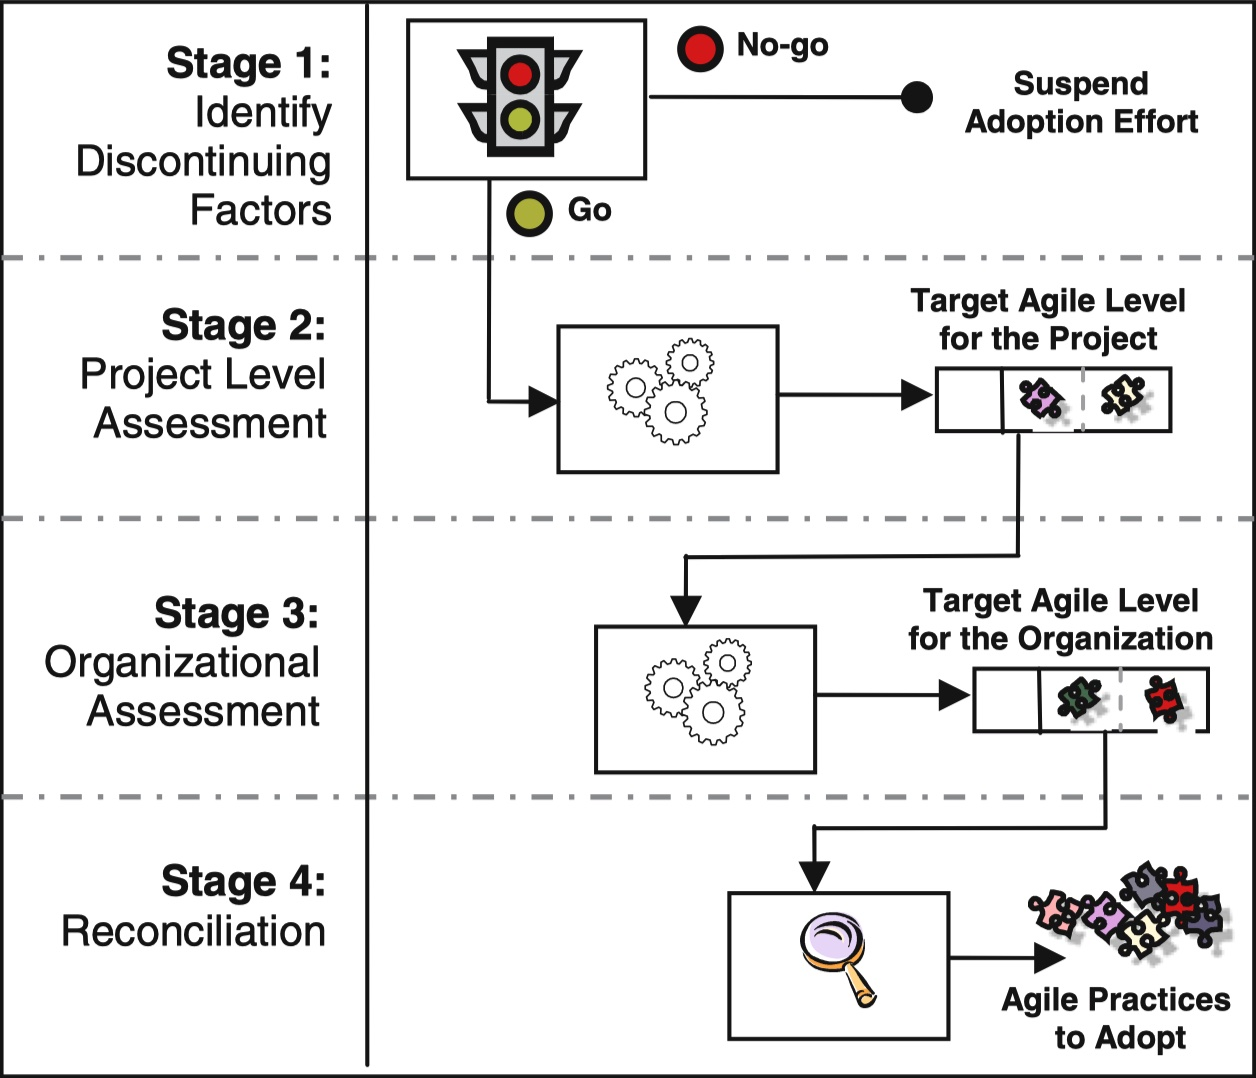
\includegraphics[width=1.0\linewidth]{img/four-stage.jpg}
    \caption{The four-stage process for agile adoption}
    \label{four-stage}
\end{figure}

在下一部分将会详细解释四阶段的每个阶段是如何帮助实现它所阐明目标。

\subsection{Making the go/no-go decision}

流程的第一个目标是提供给企业一个决定是否继续进行敏捷化采用方案的方法。由于采用敏捷实践是一种软件过程改进(SPI),因此在决定启动该计划之前需要进行预评估阶段。传统上,预评估决定了组织开展SPI计划的能力\cite{grady1997successful}。缺乏成功SPI工作所需因素的组织被认为“尚未准备好”。在这种情况下,SPI工作暂停直到缺失的因素被满足。

同样,在敏捷采用方面,预评估有助于识别组织中可能阻碍成功采用敏捷实践的因素。 如果存在这些因素,组织必须在继续采用之前消除它们。 像这样的预评估流程很重要,因为它们可以通过识别可能导致SPI计划失败的前期缺失或现有因素来节省组织时间,金钱和工作量\cite{jan2005aim}。

下一节将介绍流程的第1阶段如何指导和帮助组织制定关于采用敏捷实践的决策/不制决策。 该决定由确定任何中断因素的预评估活动决定。

\subsubsection{Stage 1: Identifying discontinuing factors}

第1阶段的目的是提供一个评估过程,确定可能阻碍成功采用敏捷实践的关键因素。 这些被称为中断因素,它们因组织而异。 通常,它们与组织的资源有关,包括金钱,时间和工资,以及对领导者的支持。 以下是敏捷采用框架确定的三个中断因素:

\begin{itemize}
    \item[$\bullet$] \textit{对敏捷性的不恰当需求:}这指的是从业务或软件开发的角度来看,采用敏捷性不会增加任何价值的情况\cite{spayd2003evolving}。
    \item[$\bullet$] \textit{缺乏足够的资金:}如果资金不可用或不足以支持敏捷采用工作,那么采用流程就不可行。
    \item[$\bullet$] \textit{缺乏行政支持:}如果没有来自执行发起人的承诺支持,那么组织中的有效和实质性变化就不太可能发生\cite{pukinskis5stumbling,spayd2003evolving}。
\end{itemize}

当一个组织展示出任何这些中断因素时,它没有准备好向敏捷性迈进,应该暂停采用流程,直到环境更具支持性。

关注组织特征的指标用于评估组织中存在中断因素的程度。评估员使用一个或多个指标来评估每个组织特征。 例如,可以衡量以确定是否缺乏足够资金的两个组织特征是(1)分配给流程改进工作的美元金额和(2)实际花费资金用于敏捷采用的能力。用于评估在敏捷采用上花费资金的能力的问题(指标)的一个例子是资金可以用于任何流程改进活动吗?另一个评估问题是,对这些资金可以使用的活动类型是否有任何限制?敏捷采用框架中包含20多个指标,用于评估组织中存在的中断因素\cite{sidky2006agile}。

\subsection{Identify agile practices to adopt}

如果第1阶段表明组织已准备好向敏捷性迈进,那么将敏捷实践引入开发过程的过程就开始了。 这涉及确定哪些敏捷实践和概念最适合组织采用。 实际上,更准确地说,敏捷采用框架首先决定了特定项目可以采用的敏捷实践,而不是整个组织。 该框架基于这样一种基本信念:组织中的每个项目都可以根据其上下文采用不同程度的敏捷性。 因此,最后三个阶段为确定适合单个项目的敏捷实践提供了指导:

\begin{itemize}
    \item[$\bullet$] \textit{第2阶段:项目等级评估:}确定项目可达到的最高敏捷化水平。 这也称为目标敏捷级别。
    \item[$\bullet$] \textit{第3阶段:组织准备评估:}确定组织准备好适应项目目标敏捷级别的程度。
    \item[$\bullet$] \textit{第4阶段:协作。}解决项目可以采用的最高敏捷性与组织准备接受的敏捷性之间的差异(如果有的话),并确定要采用的敏捷实践。
\end{itemize}

% TODO

\subsubsection{Stage 2: Project level assessment}
\label{section3.2.1}

第2阶段是采用过程的第一阶段,利用前面提到的SAMI。此阶段的目标是确定项目可以实现的最高级别的敏捷性。 这称为目标级别,是五个敏捷级别之一。

从理论上讲,所有项目都应该立志达到最高水平的敏捷性。然而,现实情况是,通常在组织控制之外的环境围绕着每个项目。 如果这些情况对组织采用敏捷实践的能力产生不利影响,则会成为制约因素。因此,约束因素限制了项目所期望的敏捷性水平。

例如,\textit{频繁的面对面交流}是第3级的理想敏捷实践。成功采用这种做法所需的一个因素是靠近团队。 假设项目和组织在改变这个项目特征(即因素)方面没有发言权,因为它超出了他们的控制范围。 如果项目级别评估确定此项目缺少该因素(靠近团队邻近度),那么此项目的最高敏捷性将与发现此敏捷实践的敏捷级别相同(在这种情况中是级别3)。

因为实现最高级别的敏捷性取决于组织控制之外的项目环境,所以项目级别评估的第一步是确定那些依赖于这些环境以成功采用的敏捷实践和概念。这些敏捷实践被称为\textit{限制敏捷实践},因为如果不支持这些实践所需的项目特征,则无法采用该实践会限制或限制项目可达到的敏捷性级别。 在表1中说明SAMI的情况下,限制敏捷实践有下划线。

第2阶段定义的评估过程侧重于确定项目的目标敏捷性水平。更具体地说,它仅检查与限制敏捷实践相关的那些因素,并测量它们存在的程度。评估是使用与每个限制敏捷实践相关的指标进行的。该过程首先检查敏捷级别1的限制性实践,然后按比例向上移动。一旦发现采用限制性做法所需的因素缺失,评估过程就会停止,项目可达到的最高敏捷度将被设定为发现限制性做法的水平。

总之,敏捷性的目标水平是在评估过程发现缺少采用限制敏捷实践或概念所需的项目特征之一时确定的,项目和组织都无法做任何事情来影响或改变这一点。 环境。 在确定项目的目标敏捷级别之后,行程的下一步是进行组织准备评估,以确定可以采用的敏捷实践(针对项目)。

\subsubsection{Stage 3: Organizational readiness assessment}
\label{section3.2.2}

确定项目的目标级别并不一定意味着该级别是可实现的。为了确定可以达到目标水平的程度,必须对组织进行评估,以确定是否已准备好采用与目标水平相关的每个敏捷实践和概念。在每种敏捷实践的此类预采用评估中投入时间和精力可以提高整体向敏捷过渡的成功概率\cite{boehm2005management},因为它可以显着降低与敏捷采用过程相关的风险。

与阶段2类似,该过程的第3阶段也依赖于Sidky敏捷测量指数(SAMI)。指标在确定目标水平达到的程度方面发挥着关键作用。 为了在此评估阶段节省时间和金钱,而不是评估组织在采用所有敏捷级别的实践方面的准备程度,而只使用目标敏捷级别及以下级别的组织。评估员使用与敏捷实践相关的一组指标(问题)来衡量每种组织特征的存在程度。

例如,\textit{协作}计划是第1级中的敏捷概念。为了评估组织采用此概念的准备情况,以下是需要提供的一些组织特征:(a)协作管理方式,(b)管理支持采用敏捷实践,(c)管理透明度,(d)组织中的小功率距离,以及(e)开发人员支持采用敏捷实践。

使用许多不同的问题评估这些组织特征中的每一个。根据问题,组织内的经理或开发人员或评估员自己应答。 SAMI包含大约300个指标,用于衡量与敏捷实践和概念相关的各种组织特征\cite{sidky2006agile}。

组织评估阶段的结果是一个表格,描述了每个组织特征的实现程度(见表\ref{table2})。这种显示结果的格式对高管和决策者有利,因为它提醒人们注意可能导致采用实践失败的组织特征。类似于项目级评估,确定组织能够实现的最高敏捷级别取决于组织是否愿意采用敏捷级别的实践。如果发现实践所需的组织特征未能实现或仅部分实现,那么这表明组织尚未准备好采用该实践。因此,组织可以达到的最高敏捷性水平成为缺少必要组织特征的水平。例如,在表2中,由于协作计划处于敏捷级别1,并且由于其所需的两个特征是有缺陷的,因此该组织的最高级别的敏捷性是级别1。

\begin{table}[htb]
    \centering
    \caption{Organizational assessment results}
    \label{table2}
    \begin{tabular}{|m{0.2\linewidth}|m{0.26\linewidth}|m{0.05\linewidth}|m{0.05\linewidth}|m{0.05\linewidth}|m{0.05\linewidth}|}
        % >>> row 1
        \hline
        \multicolumn{1}{|C|}{敏捷实践} & \multicolumn{1}{C|}{必要的组织特征} & \multicolumn{1}{C|}{NA} & \multicolumn{1}{C|}{PA} & \multicolumn{1}{C|}{LA} & \multicolumn{1}{C|}{FA} \\ \hline
        
        % >>> row 2
        反思和调整 & ... & & & & \\ \hline
        
        % >>> row 3
        \multirow{5}{*}{\textbf{协作计划}} & 透明化管理 & & & X & \\ \hhline{|~|-----|}
        
        % >>> row 4
        & 组织中的权利差距小 & & & & X \\ \hhline{|~|-----|}
        
        % >>> row 5
        & 雇佣开发者 & & & & X \\ \hhline{|~|-----|}
        
        % >>> row 6
        & 协作管理风格 & & X & & \\ \hhline{|~|-----|}
        
        % >>> row 7
        & 雇佣管理者 & X & & & \\ \hline
        
        % >>> row 8
        标准化编程 & ... & & & & \\ \hline
    \end{tabular} \\ \vskip .2cm
    \textbf{NA:} 没有完成(0\%-35\%)   \textbf{PA:} 部分完成(35\%-65\%) \\ \vskip .2cm
    \textbf{LA:} 大部分完成(65\%-85\%)   \textbf{FA:} 全部完成(85\%-100\%)
\end{table}

\subsubsection{Stage 4: Reconciliation}
\label{section3.2.3}

在组织准备评估之后,组织可实现的敏捷级别是已知的。在此之前,第2阶段确定了项目希望采用的敏捷级别。因此,确定项目将采用的敏捷实践需要最后一步,即协调。 在此阶段,解决目标级别与组织准备情况之间的差异,以确定将采用/使用的最终敏捷实践集。在此阶段可能有三种不同的情景:

\begin{itemize}
    \item[$\bullet$] \textit{组织准备级别>项目目标级别:}不需要协调,项目敏捷级别及以下的所有实践都成为选择采用的敏捷实践。 这是一种罕见的情况,因为项目环境通常包含在组织中。
    \item[$\bullet$] \textit{组织准备水平=项目目标水平:}不需要协调,项目敏捷级别及以下的所有实践都成为选择采用的敏捷实践。 这是理想的案例,因为该项目实现了100%的敏捷潜力。
    \item[$\bullet$] \textit{组织准备级别<项目目标级别:}需要进行协调。 如下所述,该框架提供了两种协调这种情况的选项。
\end{itemize}

\paragraph{选项1:}

第一种选择依赖于组织对变更和改进的准备和愿意。 组织评估的结果确切地确定了哪些特征阻碍了组织达到更高的敏捷性水平(即项目的目标水平)。 如果改变任何这些特征在组织的控制范围内,那么组织可以采取必要的步骤来改善这些特征。 成功完成所有建议的更改后,组织可以在项目的目标级别支持敏捷实践。

\paragraph{选项2:}

第二种选择适用于不愿意为变革投入时间,精力或资金的组织,并且只希望采用当前能力范围内的敏捷实践。在这种情况下,建议仅采用组织准备好的敏捷实践。 这种方法的明显缺点是该项目仅限于以低于其潜力的敏捷性运行。

此协调阶段可帮助组织切实识别其可采用的敏捷实践。同时,如果组织能够并且愿意改进,那么这个阶段就会指导它需要改进的地方,以便项目能够以其充分的敏捷潜力运作。此外,通过利用这种方法,组织在开始将敏捷实践引入开发过程之前充分准备自己,从而减少采用过程的影响。

下一节简要概述了敏捷社区对敏捷采用框架的证实所收集的结果。

\section{Quantitative feedback on the agile adoption framework}

纵向研究是验证敏捷采用框架的理想方法。特别是,将实施敏捷采用框架的组织中的开发过程与不实现敏捷采用框架的组织中的开发过程进行比较,可以生成证实框架有效性所需的经验证据。然而,这类研究面临的挑战是需要大量的时间和资金。此外,为了收集足够的经验证据,多个组织必须同意参与。 后一种要求加剧了这一问题,因为大多数组织对采用新的框架犹豫不决,而且没有任何验证证据。

因此,我们选择通过向敏捷社区成员提供框架的“优点”而不是纵向研究,并就其目标和实现这些目标的能力引出反馈。更具体地说,敏捷采用框架已提交给敏捷社区的28个成员。在与参与者(或其中一组)的90分钟个人访问中收集反馈,其中包括框架,讨论和完成问卷的一段时间的介绍。 本部分其余部分提供了反馈的结果,并从两个角度展示:参与者的角色或位置,以及他们的经验年数。此外,SAMI的反馈与四阶段过程的反馈分开。

\subsection{Results for the SAMI}

关于SAMI的问题涉及对其全面性,实用性,必要性以及实践是否处于适当水平的反馈。

\begin{figure} [htb]
    \centering
    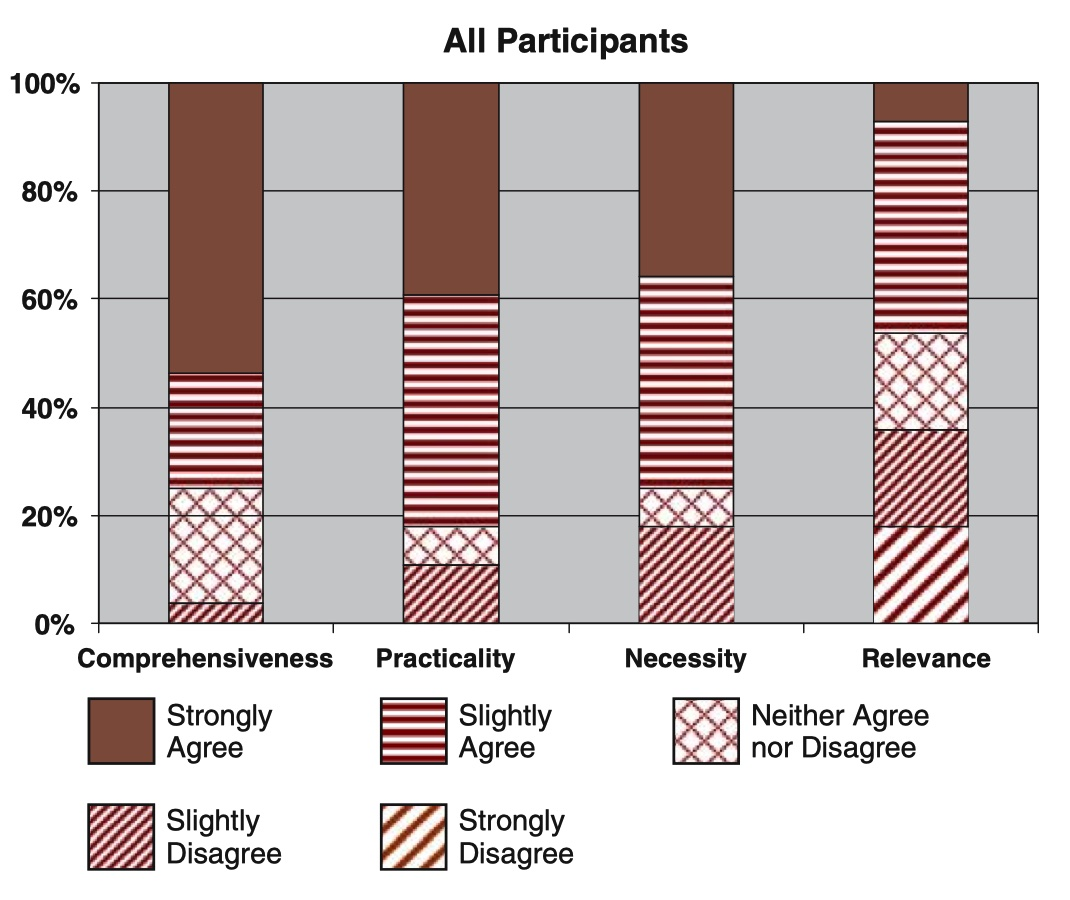
\includegraphics[width=1.0\linewidth]{img/feedback.jpg}
    \caption{Overall feedback about the SAMI}
    \label{fig.4}
\end{figure}

图\ref{fig.4}表明,超过75%的受访者同意或非常同意SAMI是全面,实用和必要的。 但是,对敏捷实践与其所定义的敏捷级别的相关性问题的回答表明,协议率降至50%以下,而分歧率则上升至约37%; 其余的受访者既不同意也不反对。

\begin{figure*} [htb]
    \centering
    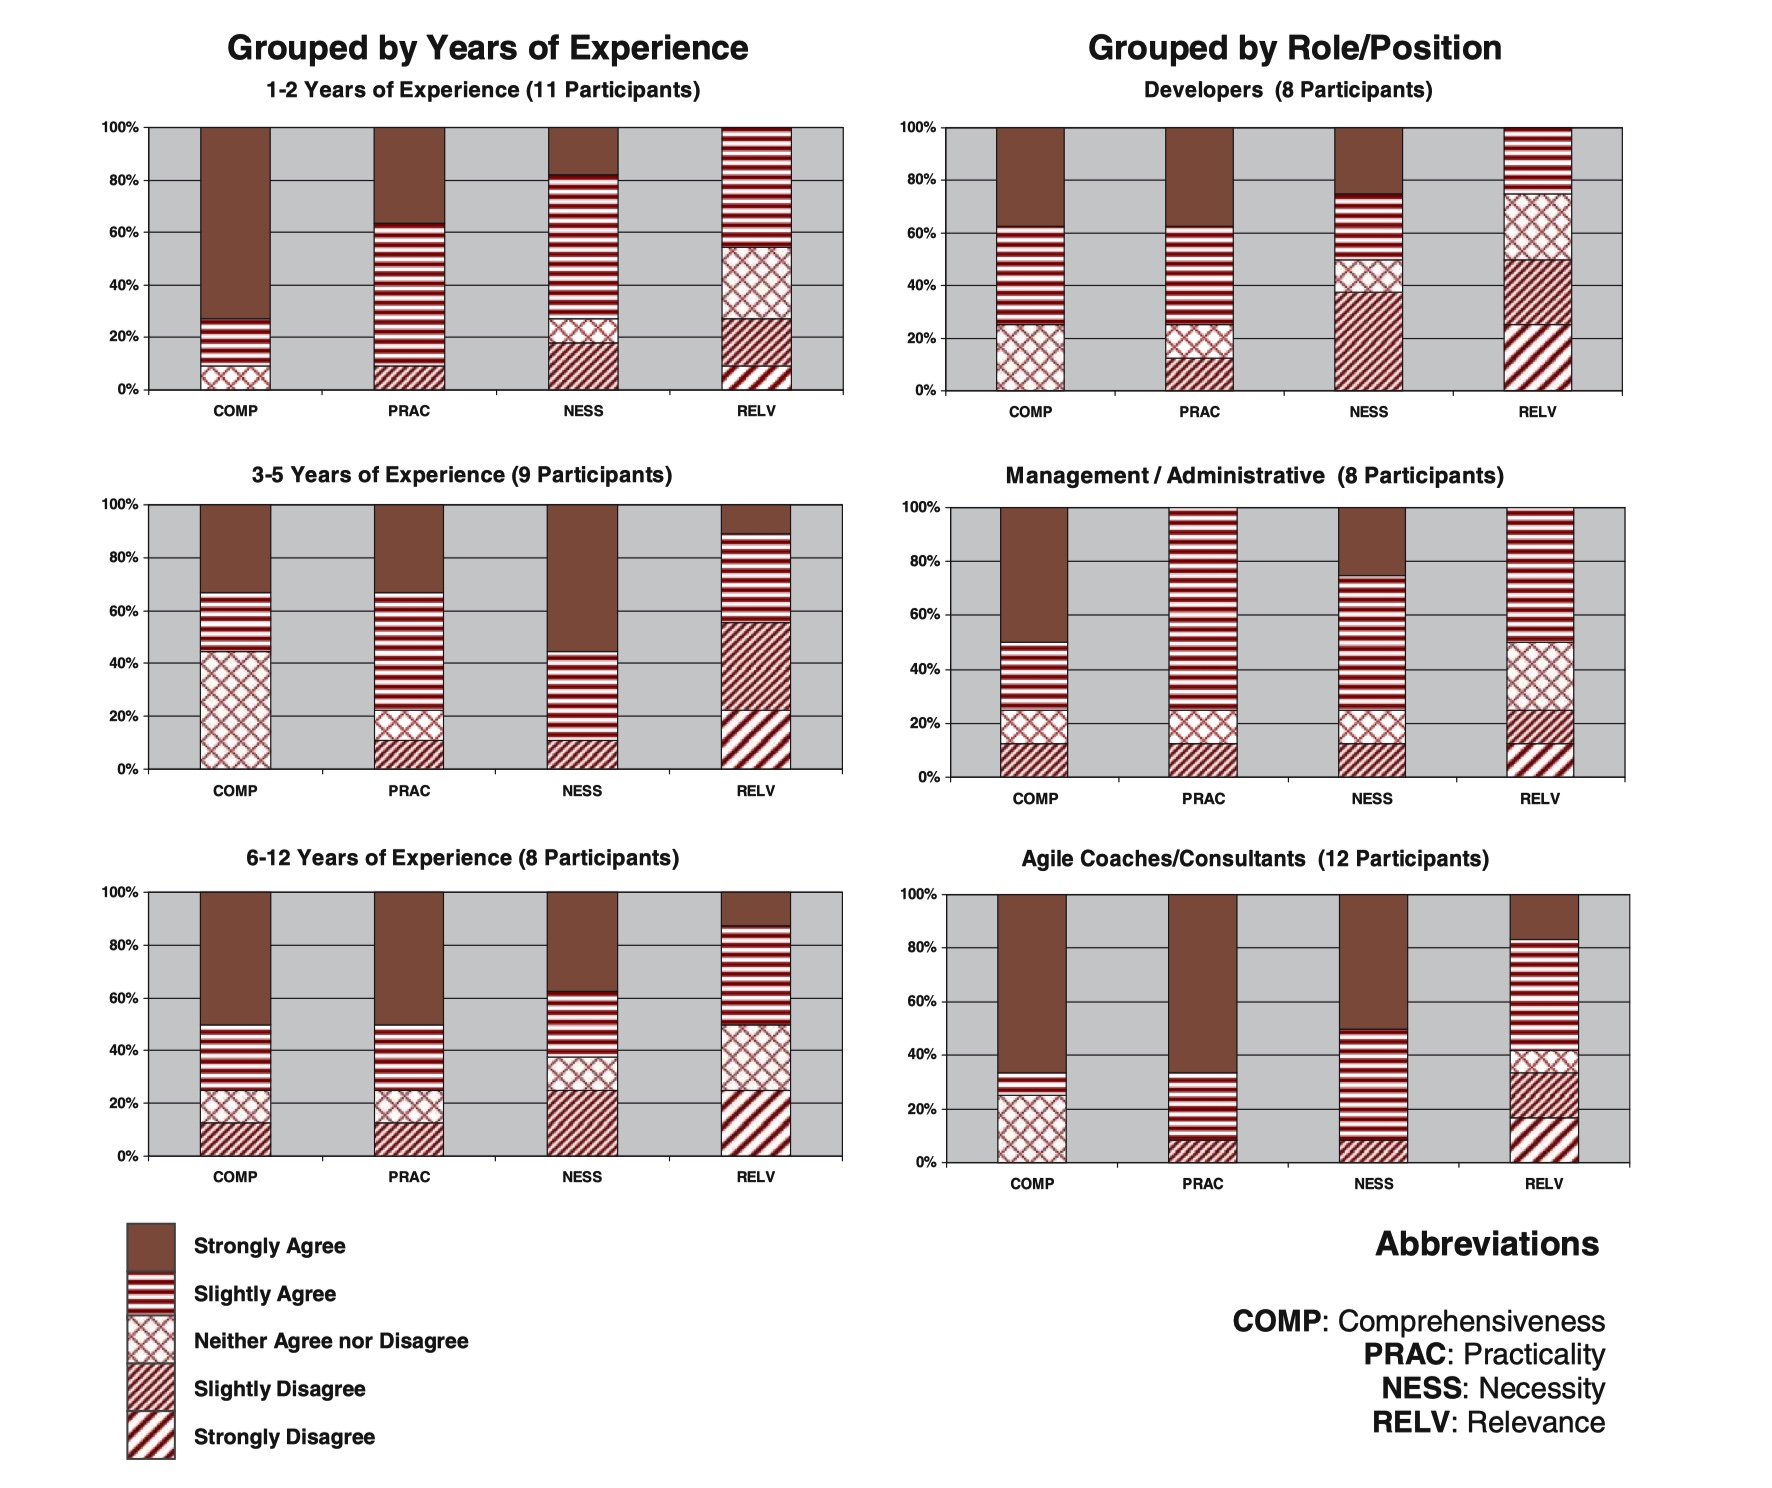
\includegraphics[width=1.0\textwidth]{img/fig5.jpg}
    \caption{Results of the SAMI grouped by role and experience}
    \label{fig.5}
\end{figure*}

为了进一步分析,图\ref{fig.5}提供了参与者经验和角色(开发人员,管理人员和教练/顾问)对总体数据的细分。 如图所示,反馈主要与SAMI的全面性,实用性和必要性一致。

但是,参与者之间在相关性方面存在一些差异。 最突出的问题是敏捷实践在各级内的地位。 我们推测这是因为每个参与者都有不同的经历,这取决于他们的角色,多年的经验以及他们参与的项目。 随后,每个参与者对实践的使用给予不同的优先权。 这种有益的反馈和随后的洞察力使我们认识到灵活性的实用性和必要性,以便定制SAMI以实现(a)个人经验,或许(b)业务目标。

在根据参与者角色检查结果时,同样重要的是要注意敏捷教练和顾问一般比其他角色的参与者有更多的积极反馈。

最后,基于对全面性,实用性和必要性的考察,图\ref{fig.5}表明确实需要有关如何组织这些敏捷实践和概念的结构和指导 - 事实上,这正是SAMI旨在提供的内容和指导。

\begin{figure} [htb]
    \centering
    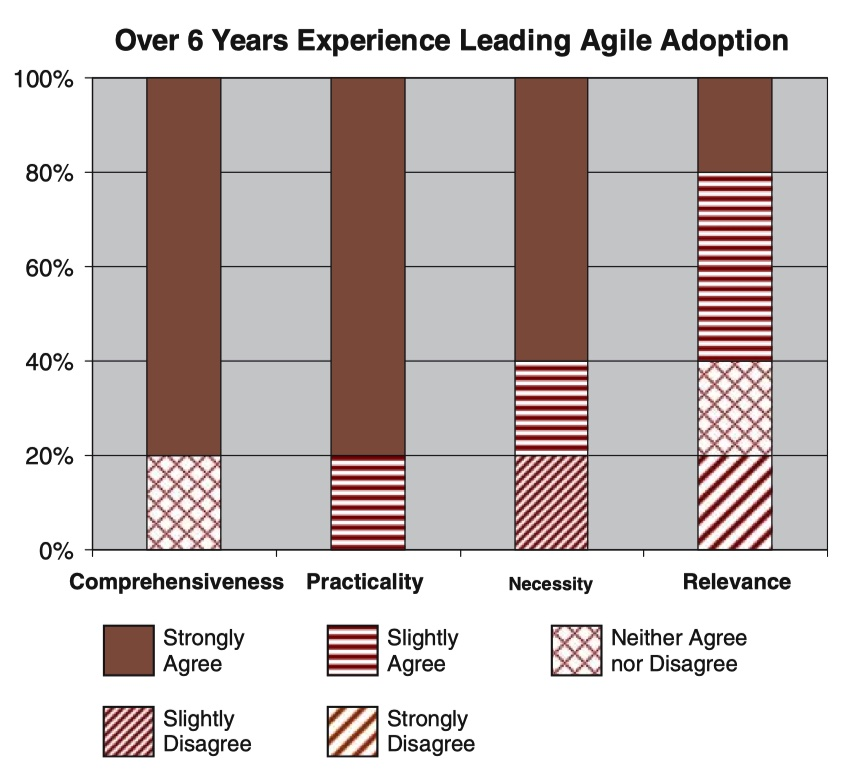
\includegraphics[width=1.0\linewidth]{img/fig6.jpg}
    \caption{Feedback about the SAMI from participants with over 6years of experience leading agile adoption efforts}
    \label{fig.6}
\end{figure}

图\ref{fig.6}总结了在领导敏捷采用工作方面拥有超过六年经验的参与者的反馈。 图中显示,80%的这些专家非常同意SAMI定义的敏捷级别的全面性,而剩下的20%既不同意也不反对。 他们都同意敏捷程度的实用性,80%表示强有力的支持。 此外,80%同意灵活性水平的必要性,而只有20%略微不同意。 至于实践与水平的相关性,60%的人认为这些做法或多或少处于正确的水平,而20%的人选择保持中立,直到他们更彻底地研究了五个水平。 剩下的20%强烈不同意。

总之,敏捷社区认识到SAMI的实用性和需求。 这很重要,因为它是四阶段采用过程的基础组成部分。 下一节将介绍有关四阶段流程(敏捷采用框架的主要组成部分)的反馈。

\subsection{Results for the four-stage process}

\begin{figure} [htb]
    \centering
    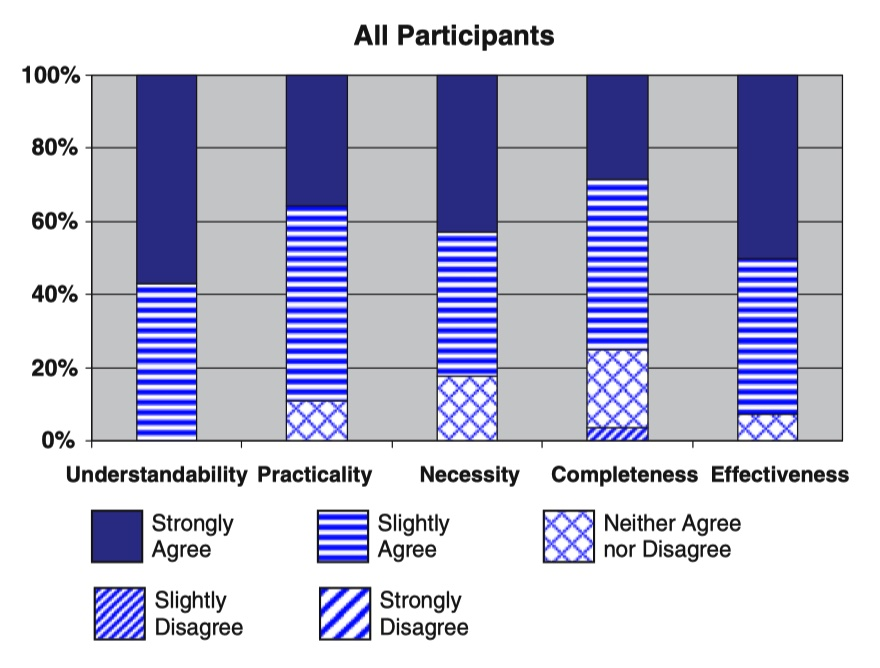
\includegraphics[width=1.0\linewidth]{img/fig7.jpg}
    \caption{Overall feedback about the four-stage process}
    \label{fig.7}
\end{figure}

图\ref{fig.7}描绘了相对于四阶段过程的总体反馈。 该反馈侧重于四阶段过程的可理解性,实用性,必要性,完整性和有效性。 如图所示,大多数参与者(约80%)同意或强烈同意上述所有五个特征。 有希望的是,没有一个参与者强烈反对四阶段过程的任何方面,只有一个参与者略微不同意其完整性。

\begin{figure*} [htb]
    \centering
    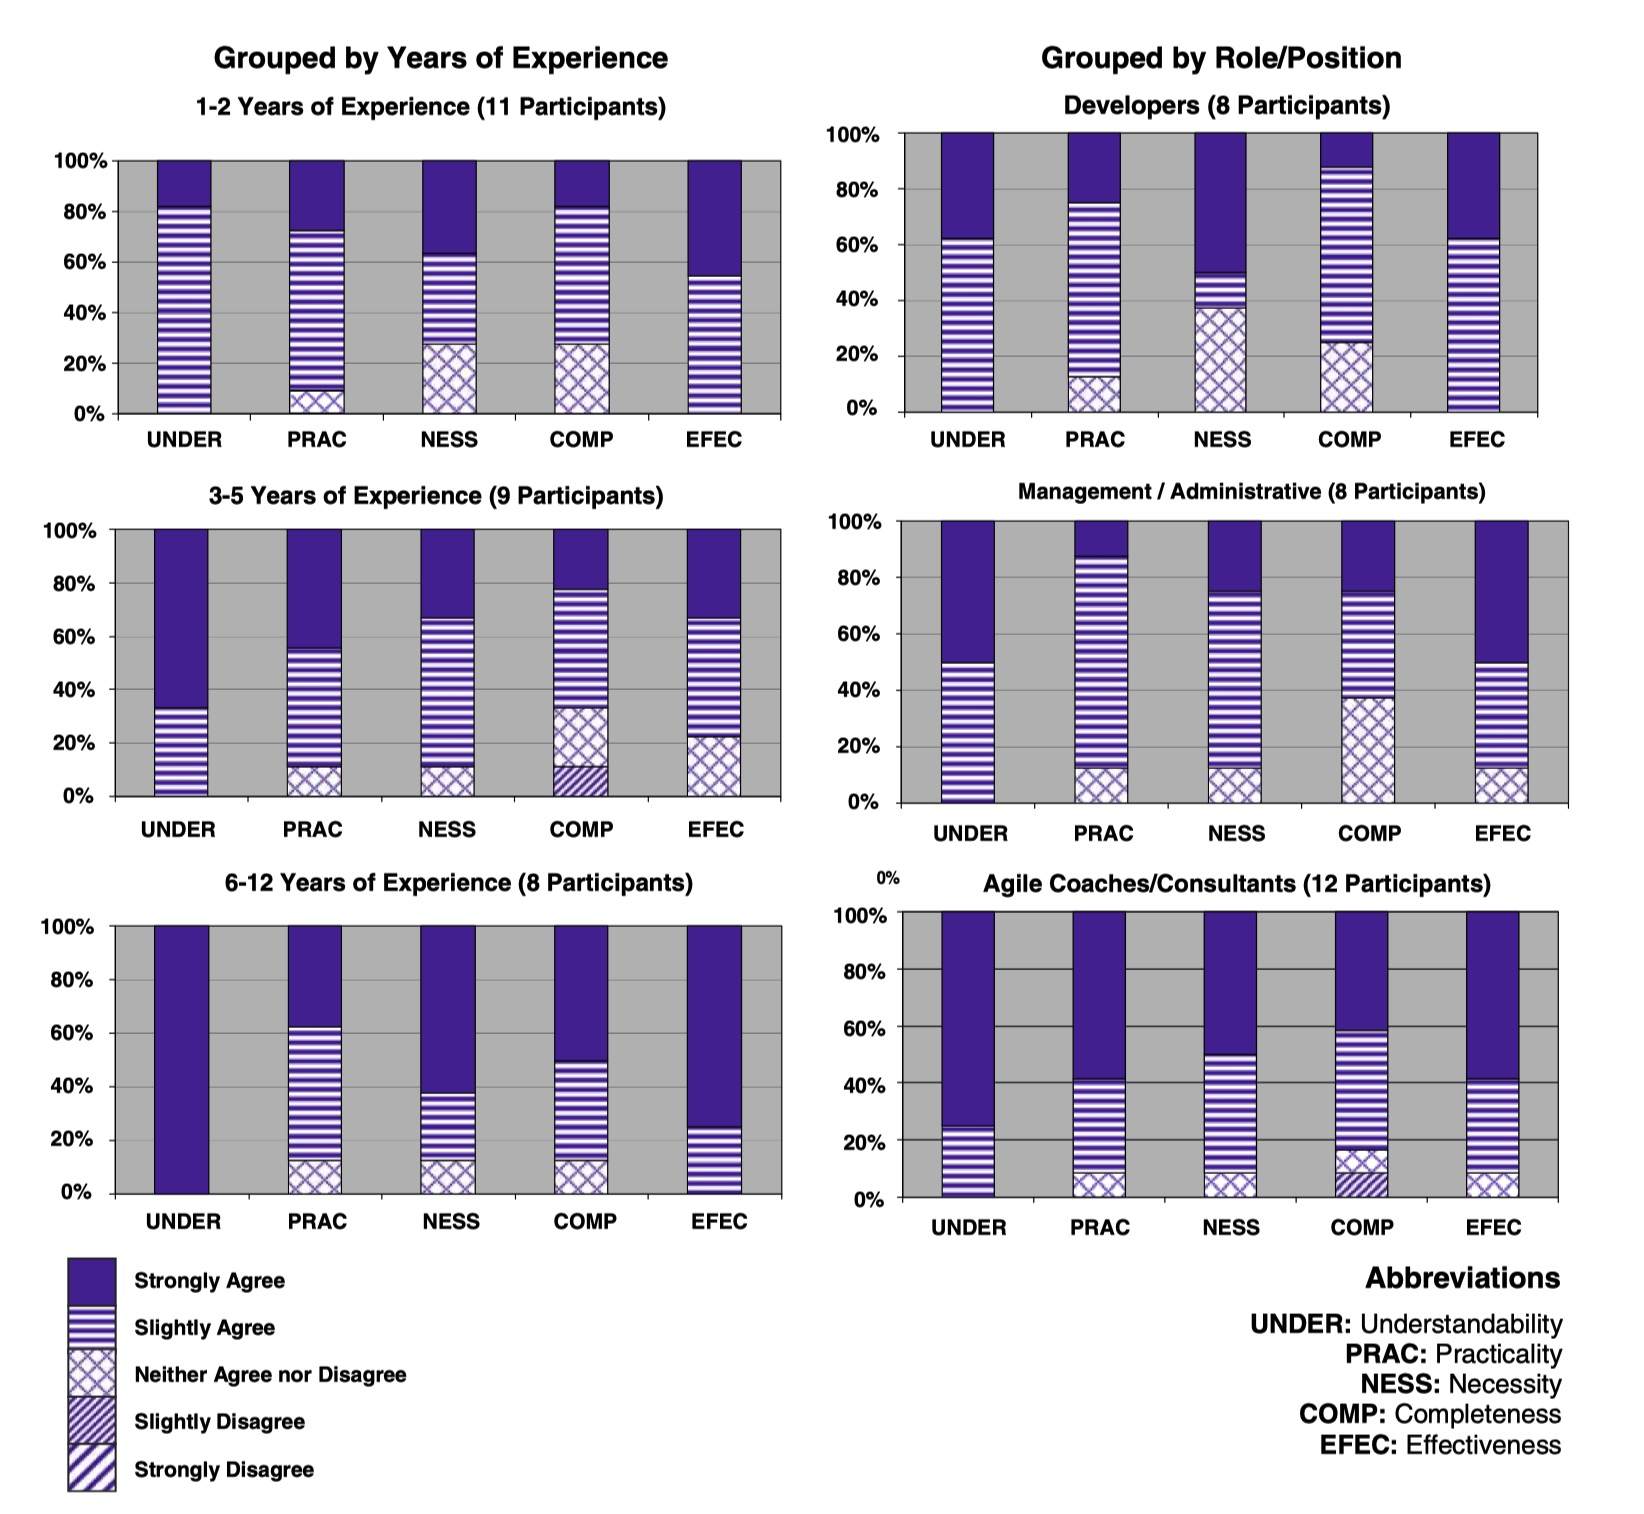
\includegraphics[width=1.0\textwidth]{img/fig8.jpg}
    \caption{Results of the four-stage process grouped by role and experience}
    \label{fig.8}
\end{figure*}

图\ref{fig.8}按年经验和角色提供了参与者的细分。从描述中,我们注意到协议级别与经验年限和个人角色成正比:敏捷采用的经验和直接参与越多,协议等级越高。特别是,所有经验丰富的人都非常同意这个过程清晰易懂。这是预期的,因为该过程旨在为其特定活动建模。与该过程的其他方面相比,四阶段过程的完整性具有最低的协议百分比。我们推测,造成这种情况的一个主要因素是用于收集反馈的过程。特别是,只有90分钟的时间用于向参与者提供框架,进行后续讨论并进行调查。我们希望这个时间段太短,参与者(或任何人)无法完全掌握完整框架的本质以及其组成部分之间的实质关系。这种期望在某种程度上得到了参与者的肯定,这些参与者在稍后时间(不是在演示之后立即)返回问卷 - 他们都强烈同意四阶段过程完成。

\begin{figure} [htb]
    \centering
    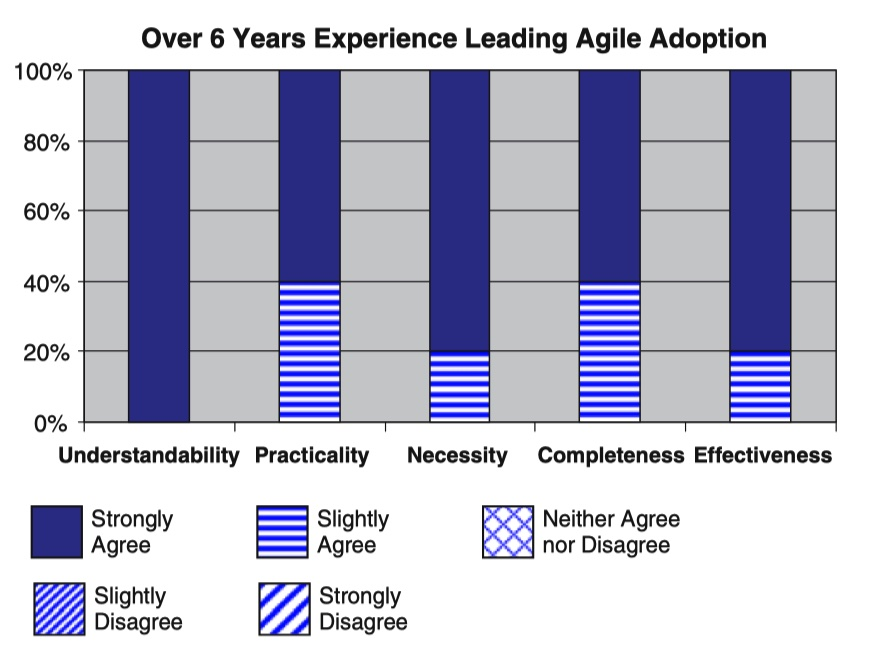
\includegraphics[width=1.0\linewidth]{img/fig9.jpg}
    \caption{Feedback about the four-stage process from participants with over 6years of experience leading agile adoption efforts}
    \label{fig.9}
\end{figure}

图\ref{fig.9}总结了从具有超过6年领导敏捷采用工作经验的参与者收集的四阶段流程的反馈。 对这些结果真正值得注意的是,这组专家中有100%同意所调查的四阶段过程的所有五个方面(可理解性,实用性,必要性,完整性和有效性)。 这些结果强调了四阶段过程的感知效用,并有助于证实其有效性。

最后,从演示,讨论和调查中获得的反馈往往表明(并且证实了我们自己的看法)敏捷采用框架(四阶段过程和SAMI)尚未充分发挥其潜力。 尽管如此,我们对收到的关于敏捷采用框架的一些定性评论感到鼓舞:

\begin{itemize}
    \item[$\bullet$] “我认为这很棒(工作)” —— 具有12年经验的敏捷顾问
    \item[$\bullet$] “这是这项工作的正确时间!优秀的工作“ —— 具有8年经验的敏捷顾问
    \item[$\bullet$] “总的来说,这是一流的工作,我赞同这项工作对我们的行业的利益和价值是合法的” —— XP教练有6年的经验
\end{itemize}

\section{Conclusion}

敏捷采用框架是解决为组织提供结构化和可重复的方法以指导和协助他们实现敏捷性的需求的第一步。该框架独立于任何一种特定的敏捷方法或样式,在框架内使用XP或SCRUM或任何其他敏捷样式没有任何限制。此外,该框架有两个级别的评估:一个在项目层面,另一个在组织层面。因此,它适应每个项目的独特性,同时认识到每个项目都是一个整体组织所包围的,并且是整个组织的一部分,必须准备好采用必要的敏捷实践。我们将敏捷采用框架视为回答如何采用敏捷实践的复杂问题的初步贡献。总之,我们建议将此框架作为指导和协助组织采用敏捷实践的方法。通过识别和评估中断因素的存在,组织可以做出关于敏捷性转变的决定/不做决定。通过确定项目的目标水平,然后评估组织以确定其准备好达到目标敏捷水平的程度,该框架设法为教练提供一套切实可行的敏捷实践,供项目采用。通过使用SAMI,四阶段过程评估提供了在采用工作开始之前需要改进的组织内部区域的广泛概述。

\bibliographystyle{spmpsci}
\bibliography{mybibtex}

\end{document}

